% 刚体的平面运动方程

\pentry{质心\ 质心系\upref{CM}, 动量定理\upref{PLaw},转动惯量\upref{RigRot}}

任意惯性系中,若刚体质量为 $M$,质心为 $\vec r_c$,刚体受若干个力 $\vec F_i$,作用点分别为 $\vec r_i$,若刚体\bb{只延一个固定的方向转动}(如刚体的二维运动),且该方向关于质心的转动惯量为 $I$, 则质心运动方程和绕质心转动的方程分别为
\begin{equation}\label{RBEM_eq1}
M\vec a_c = \sum_i \vec F_i
\end{equation}
\begin{equation}\label{RBEM_eq2}
I \vec \alpha = \sum_i \vec \tau_i = \sum_i (\vec r_i-\vec r_c) \cross  \vec F_i
\end{equation}
其中 $\vec a_c$ 是质心的加速度, $\vec \alpha$ 是绕质心转动的角加速度.这是说,我们可以把刚体的运动分解成质心的移动和相对质心的转动,并用合力计算前者,用关于质心的合力矩计算后者.

\subsection{推导}
我们把刚体看做质点系来证明,在任意惯性系中,由动量定理,刚体总动量,即质心动量 $\vec p_c$ 的变化率为
\begin{equation}
\dv{t} \vec p_c = M \vec a_c = \sum_i \vec F_i
\end{equation}

现在我们用角动量定理证明\autoref{RBEM_eq2}.由于质心与刚体的相对位置不变,%未完成:这个怎么证明啊?
质心系中刚体必须绕质心转动,且角动量为(\autoref{RigRot_eq5}\upref{RigRot}) $\vec L_c = I \vec\omega$, 角动量变化率为\footnote{注意第一步成立的条件是 $I$ 不变,而一般情况下 $I$ 与刚体的转轴有关,所以只能假设刚体延同一方向转动.唯一的例外是物体的转动惯量与方向无关的情况,例如球体.刚体的变向转动较为复杂,不做讨论.}
\begin{equation}
\dv{\vec L_c}{t} = I \dv{\vec \omega}{t} = I \vec\alpha
\end{equation}
要特别注意的是,除非合力为零,质心系并不是惯性系,所以使用角动量定理要考虑刚体的惯性力.但幸运的是质心系中惯性力(\autoref{Iner_eq5}\upref{Iner}) $-m_i \vec a_c$ 产生的合力矩为零\upref{PSys}
\begin{equation}
\sum_i \vec r_{ci}\cross (-m_i \vec a_{c}) = \vec a_{c} \cross \sum_i m_i \vec r_{ci} = \vec 0
\end{equation}
现在我们可以继续角动量定理\upref{AMLaw} 得
\begin{equation}
I \vec\alpha = \sum_i \vec r_{ci} \cross  \vec F_i
\end{equation}
由于质心系相对于任何惯性系没有相对转动, 所以在任意惯性系中刚体的角加速度仍然为 $\vec\alpha$.但受力点的位矢变为 $\vec r_i = \vec r_c + \vec r_{ci}$,即
\begin{equation}\label{RBEM_eq7}
I \vec \alpha = \sum_i (\vec r_i-\vec r_c) \cross  \vec F_i
\end{equation}

\begin{exam}{球体或圆柱延斜面无摩擦滚动}\label{RBEM_ex1}
如\autoref{RBEM_fig1}, 在一个倾角为 $\theta$ 的斜面上, 一个半径为 $R$ 质量为 $M$ 的均匀 的球体(或圆柱)从静止开始向下滚动, 其转动惯量为 $I$, 求质心的加速度和滚动的角加速度.

\begin{figure}[ht]
\centering
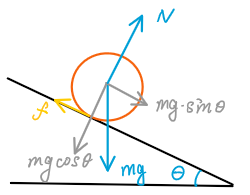
\includegraphics[width=5.3cm]{./figures/RBEM1.png}
\caption{圆柱延斜面无摩擦滚动} \label{RBEM_fig1}
\end{figure}

解: 首先, 根据无摩擦的条件, 系统只有一个自由度\upref{DoF}, 即圆柱的位移或者转角, 二者的关系为
\begin{equation}
s = R\theta
\end{equation}
两边求二阶导数, 得加速度与角加速度的关系为
\begin{equation}\label{RBEM_eq3}
a = R\alpha
\end{equation}

受力分析如图, 圆柱受三个力: 重力, 支持力和静摩擦力。 将物体受到的重力分解为垂直斜面方向和沿斜面方向的两个分力. 其中垂直方向的分力与斜面提供的支持力抵消, 而平行方向的分量和摩擦力的合力决定质心的加速度\autoref{RBEM_eq1}
\begin{equation}\label{RBEM_eq4}
mg\sin\theta - f = Ma
\end{equation}
再来分析关于质心的转动, 由于重力和摩擦力都在质心, 所以对合力矩贡献为 0。 所以只有摩擦力的贡献为 $\tau = fR$, 由\autoref{RBEM_eq2} 得
\begin{equation}\label{RBEM_eq5}
I\alpha = f R
\end{equation}
由\autoref{RBEM_eq3}到\autoref{RBEM_eq5} 三式解得加速度为
\begin{equation}
a = \frac{g \sin\theta}{1 + I/(MR^2)}
\end{equation}
可见转动惯量为 0 时, 结果与无摩擦滚动一致。 而转动惯量越大, 加速度就越小。
\end{exam}

% 未完成: 哪里讨论一下刚体运动的能量如何拆分成平动动能和转动动能两个部分?
% \begin{exam}{}
% 我们还可以从能量的角度来分析\autoref{RBEM_ex1}, 
% \end{exam}

\begin{exam}{}
一根质量为 $M$ 长为 $L$ 的均匀细棒延 $y$ 方向静止放置在水平面 $xy$,从 $t=0$ 时起在其上端施加一个 $x$ 方向的恒力,描述细棒如何运动.如果木棒与地面的摩擦系数为 $\mu$,答案又如何?

首先考虑质心的运动, 细棒所受外力只有一个恒力, 所以由\autoref{RBEM_eq1} 质心沿 $x$ 方向做匀加速运动. 再来看质心系中细棒的转动由“ 转动惯量\upref{RigRot}” 中\autoref{RigRot_ex1} 可知细棒绕其质心做单摆运动.
% 未完成: 分析有摩擦的情况
\end{exam}
